
\documentclass[12pt, a4paper]{article}
\usepackage{fullpage}
\usepackage{graphicx}
\usepackage{wrapfig}
\usepackage{amsmath}
\usepackage{float}
\usepackage{listings}
\usepackage{lmodern}  % for bold teletype font
\usepackage{xcolor}   % for \textcolor

\definecolor{codegreen}{rgb}{0,0.6,0}
\definecolor{codegray}{rgb}{0.5,0.5,0.5}
\definecolor{codepurple}{rgb}{0.58,0,0.82}
\definecolor{backcolour}{rgb}{0.95,0.95,0.92}

\title{\textbf{EE2703 : Applied Programming Lab \\ Assignment 5}} % Title

\author{Potta Muni Asheesh \\ EE19B048} % Author name

\date{\today} % Date for the report

\begin{document}	
\lstset{
  language=Python,
  backgroundcolor=\color{backcolour},   
  commentstyle=\color{codegreen},
  keywordstyle=\color{magenta},
  numberstyle=\tiny\color{codegray},
  stringstyle=\color{codepurple},
  basicstyle=\ttfamily,
  breakatwhitespace=false,         
  breaklines=true,                 
  captionpos=b,                    
  keepspaces=true,                 
  %numbers=left,                    
  %numbersep=5pt,                  
  showspaces=false,                
  showstringspaces=false,
  showtabs=false,                  
  tabsize=2,
  columns=fullflexible,
  frame=single,
  postbreak=\mbox{\textcolor{red}{$\hookrightarrow$}\space},
}	
		
\maketitle % Insert the title, author and date

\section{Introduction}

\paragraph*{}
One of the methods of solving the \textit{Laplace equation} is explored in this assignment. The Laplace equation relating electric potential to rate of change of charge density is considered here. The equation is
\begin{equation*}
\nabla^2 \phi = \frac{1}{\sigma} \frac{\partial\rho}{\partial t}
\end{equation*}
For DC current, the right hand side is zero, so the equation becomes a \textit{Laplace equation}.
\begin{equation*}
\nabla^2 \phi = 0
\end{equation*}
In the problem, a 1cm by 1cm metal plate is considered and a wire is soldered to the center of the plate and it is held at 1 Volt(V). One of the boundaries is grounded ($\phi = 0$) and for the remaining edges, the directional derivative of $\phi$ along the normal to the edge ($n$) is 0 ($\frac{\partial \phi}{\partial n} = 0$).

\section{Solving the Laplace equation}

\paragraph*{}
Since there are infinite points on the plate and data of infinite points cannot be stored, Number of points to sample along X and Y direction are given as  \texttt{Nx} and \texttt{Ny}. The radius of the wire in terms of number of points is also given. This results in a matrix corresponding to points on the plate. The \textit{Laplace equation} can be solved as follows
\begin{equation*}
\phi_{i,j} = \frac{\phi_{i-1,j} + \phi_{i+1,j} + \phi_{i, j-1} + \phi_{i, j+1}}{4}
\end{equation*}
The equation can be considered solved after doing sone number of iterations. It needs to be noted that the boundary conditions have to be re-established after each iteration. The number of iterations to be done is also given as \texttt{Niter}.

\paragraph*{Defining parameter values\\}
The values of parameters \texttt{Nx, Ny, radius, Niter} are taken from commandline arguments. If none given, then the following are considered by default.

\begin{lstlisting}
Nx=25 # number of points along X
Ny=25 # number of points along Y
radius=8 # radius of wire
Niter=1500 # number of iterations to perform
\end{lstlisting}

\paragraph*{}
Matrix \texttt{phi} is initialized to 0. The matrix has Nx columns and Ny rows. The rectangular coordinates of the sample points is obtained using \texttt{np.meshgrid}. The coordinates of points where the wire is attached to the plate are obtained using \texttt{np.where} and are stored in an array named \texttt{ii}.

\begin{lstlisting}
phi = np.zeros((Ny, Nx))
y = np.linspace(0.5*(Ny-1), -0.5*(Ny-1), Ny)
x = np.linspace(-0.5*(Nx-1), 0.5*(Nx-1), Nx)
X, Y = np.meshgrid(x,y)
ii = np.where(((X)*(X) + (Y)*(Y)) <= radius*radius)
phi[ii] = 1.0
\end{lstlisting}

\paragraph*{}
For loop is used to do the iterations, but rest of the operations are done using \textbf{vectorized code}. These operations include updating \texttt{phi} for the current iteration, asserting the boundary conditions and finding the maximum absolute change in the matrix. The maximum absolute change in the matrix \texttt{phi} is stored in an array named \texttt{errors} for each iteration.

\begin{lstlisting}
for k in range(Niter):
    oldphi = phi.copy()
    phi[1:-1,1:-1] = 0.25*(phi[1:-1,:-2]+phi[1:-1,2:]+phi[:-2,1:-1]+phi[2:,1:-1])
    phi[1:-1,0] = phi[1:-1,1]
    phi[1:-1,-1] = phi[1:-1,-2]
    phi[0,:] = phi[1,:]
    phi[ii] = 1.0
    errors[k] = np.max(np.abs(phi-oldphi))
\end{lstlisting}

\paragraph*{}
When the errors are plotted against number of iterations on a semi-log plot, a straight line with negative slope is obtained (see Figure 1), suggesting that the errors vary exponentially. 

\begin{align*}
log(error) &= log(A) + BN \\
\implies error &= Ae^{BN}
\end{align*}

\paragraph*{}
The parameters A and B are determined using \textit{Least square fitting}. Two fittings are done, one using all the errors and the other using only the errors after first 500 errors.

\begin{lstlisting}
M = np.zeros((Niter,2))
M[:,0] = 1
M[:,1] = np.arange(Niter)
fit1_params = lstsq(M, np.log(errors))[0]
fit2_params = lstsq(M[500:,:], np.log(errors[500:]))[0]
fit1_errors = np.exp(np.dot(M, fit1_params))
fit2_errors = np.exp(np.dot(M, fit2_params))
fit1_params[0] = np.exp(fit1_params[0])
fit2_params[0] = np.exp(fit2_params[0])
\end{lstlisting}

\paragraph*{}
Using the parameters obtained from both the fittings, the errors for number of iterations are computed and plotted along with the actual errors in Figure 1. The values of the parameter obtained are 
\begin{itemize}
\item For fit using all errors: A = 0.023705, B = -0.014195
\item For fit using errors after 500 iterations: A = 0.023788, B = -0.014198
\end{itemize}
It can be seen that magnitude of B is very small, so the error decreases very slowly in this method.

\begin{figure}
\centering
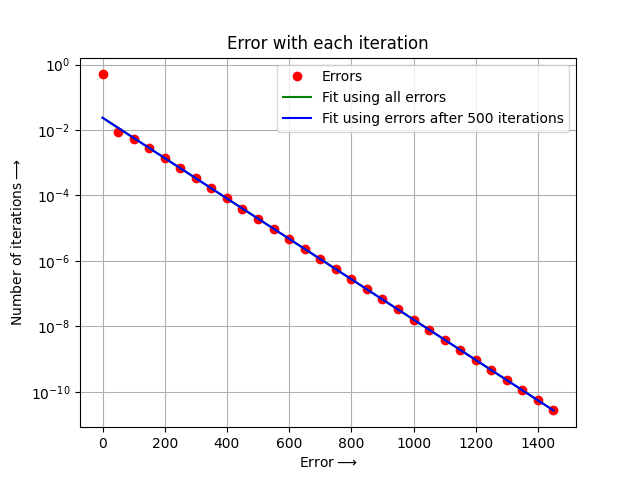
\includegraphics[width=0.8\textwidth]{Figure_1.png}
\caption{Error plot}
\end{figure}

\paragraph*{}
The 3-D surface plot of the potential and the filled contour plot of the potential are made using \texttt{plot\_surface} and \texttt{contourf} available in \texttt{mpl\_toolkits} and \\ \texttt{matplotlib.pyplot} (see Figures 2 and 3). The surface plot looks like a plateau where there is a steep decrease in potential between the wire and the grounded edge of the plate.

\begin{lstlisting}
fig2 = plt.figure(2)
ax = p3.Axes3D(fig2)
s = ax.plot_surface(X, Y, phi, rstride=1, cstride=1, cmap=cm.jet)
ax.set_xlabel(r'X$\longrightarrow$')
ax.set_ylabel(r'Y$\longrightarrow$')
ax.set_title('3-D surface plot of potential')
plt.colorbar(s, ax = ax, shrink=0.7)

plt.figure(3)
plt.contourf(X, Y, phi, (Nx+Ny)//4, cmap=cm.jet)
plt.plot(X[ii], Y[ii], 'ro')
plt.colorbar()
\end{lstlisting}

\begin{figure}
\centering
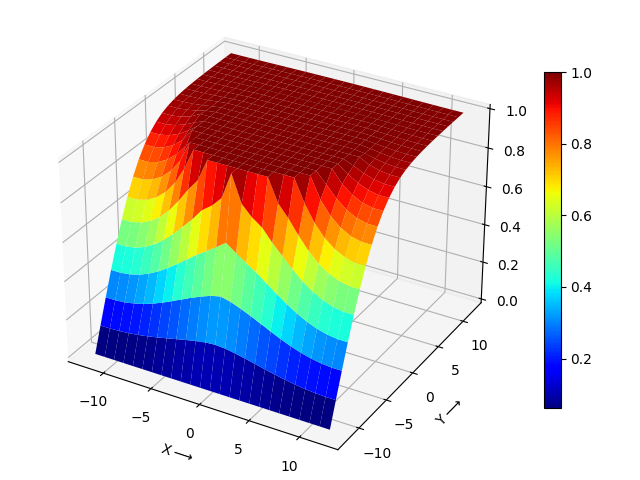
\includegraphics[width=0.8\textwidth]{Figure_2.png}
\caption{Surface plot of potential}
\end{figure}

\begin{figure}
\centering
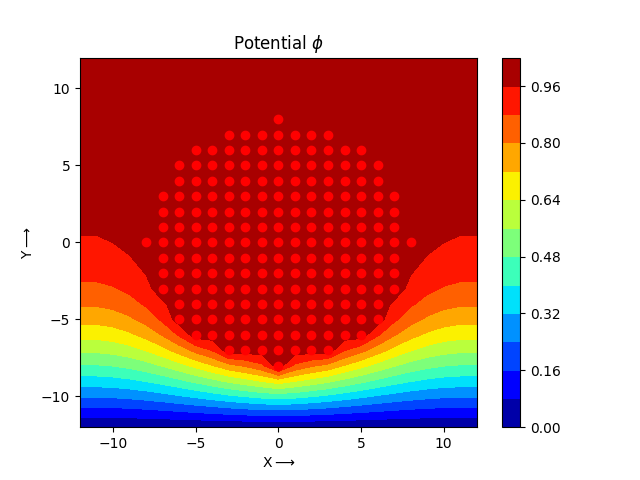
\includegraphics[width=0.8\textwidth]{Figure_3.png}
\caption{Contour plot of potential}
\end{figure}

\section{Solving for the Current density}

\paragraph*{}
From the potential, current density $\vec{j} = j_x \hat{x} + j_y \hat{y} $ can be calculated, assuming conductivity $\sigma$ = 1, as 
\begin{align*}
j_x &= -\frac{\partial{\phi}}{\partial{x}} \\
j_y &= -\frac{\partial{\phi}}{\partial{y}}
\end{align*}
Numerically, this translates to
\begin{align*}
J_{x,ij} &= \frac{\phi_{i-1,j} - \phi_{i+1,j}}{2} \\
J_{y,ij} &= \frac{\phi_{i,j-1} - \phi_{i,j+1}}{2}
\end{align*}

\paragraph*{}
Arrays \texttt{Jx, Jy} are created, which are the x and y components of the current density and the values are computed using the equations shown above as $\phi$ is known already. The vector (arrowhead) plot of the current density is made using \texttt{quiver}. 

\begin{lstlisting}
Jx = np.zeros((Ny, Nx))
Jy = np.zeros((Ny, Nx))
Jx[1:-1,1:-1] = 0.5*(phi[1:-1,:-2]-phi[1:-1,2:])
Jy[1:-1,1:-1] = 0.5*(phi[2:,1:-1]-phi[:-2,1:-1])
plt.figure(4)
plt.quiver(X, Y, Jx, Jy, scale=5)
plt.plot(X[ii], Y[ii], 'ro')
plt.title('The vector plot of current flow')
\end{lstlisting}

\begin{figure}[H]
\centering
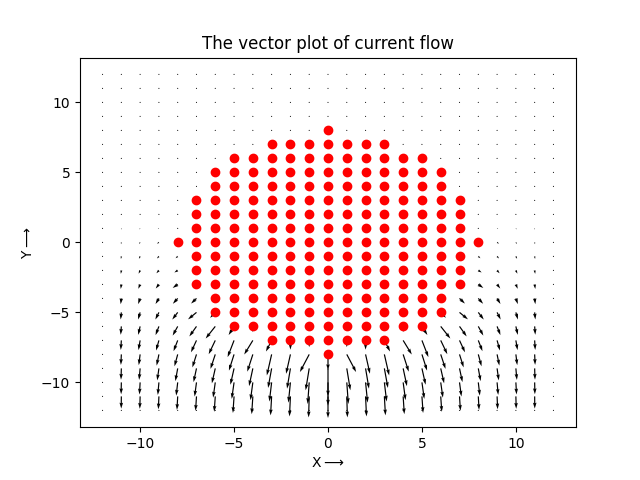
\includegraphics[width=0.8\textwidth]{Figure_4.png}
\caption{Vector plot of current density}
\end{figure}

It is observed that the current flows from the wire to the grounded edge throughout the edge at the bottom, but insignificant current flows throught top of the plate (see Figure 4). This happens because, the metal plate acts as a resistor and in a resistor, current flows from high potential zone to low potential zone only. Current flow is created due to potential difference. As there is no potential difference between points at the top, there is no current flow.

\section{Solving for temperature of the plate}

\paragraph*{}
Since the current density is known, now the temperature of the plate can be calculated from the equation given below
\begin{equation*}
\nabla \cdot (\kappa \nabla T) = -\frac{1}{\sigma} |J|^2
\end{equation*}
Assuming thermal conductivity $\kappa = 1$ and $\sigma = 1$, the equation becomes
\begin{equation*}
\nabla^2 T = -|J|^2
\end{equation*}

\paragraph*{}
Numerically, this equation translates to
\begin{equation*}
T_{i,j} = \frac{1}{4} (T_{i-1,j} + T_{i+1,j} + T_{i,j-1} + T_{i,j+1} + |J_{i,j}|^2)
\end{equation*}
The boundary conditions are given as T = 300K at the wire and the grounded edge and for the other edges, the directional derivative along normal to edge is 0. The computation is similar to the one done for potential $\phi$. The filled contour plot of temperature is plotted (see Figure 5). It is observed that heating happens only at points where current flow is more, which is intuitive.

\begin{lstlisting}
T = np.zeros((Ny, Nx))
T[:,:] = 300.0
mag_sq_J = (Jx*Jx + Jy*Jy)
for k in range(Niter):
    T[1:-1,1:-1] = 0.25*(T[1:-1,:-2]+T[1:-1,2:]+T[:-2,1:-1]+T[2:,1:-1] + mag_sq_J[1:-1, 1:-1])
    T[1:-1,0] = T[1:-1,1]
    T[1:-1,-1] = T[1:-1,-2]
    T[0,:] = T[1,:]
    T[ii] = 300.0
plt.figure(5)
plt.contourf(X, Y, T, Nx//2, cmap = cm.jet)
plt.colorbar()
\end{lstlisting}

\begin{figure}
\centering
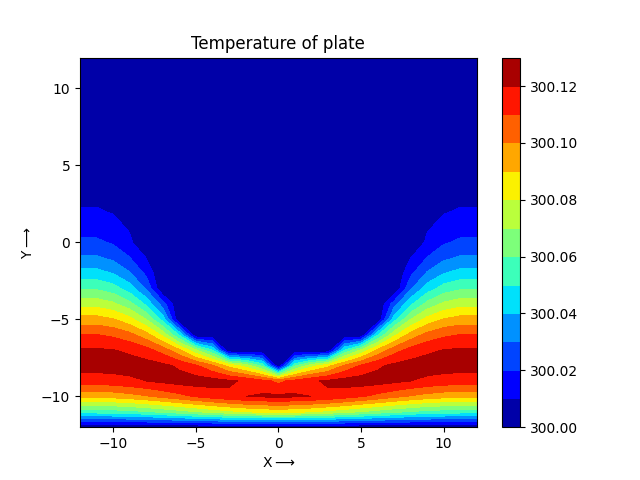
\includegraphics[width=0.8\textwidth]{Figure_5.png}
\caption{Contour plot of temperature}
\end{figure}

\section{Conclusions}
\begin{itemize}
\item Averaging method of solving Laplace (or Poisson) equation is a simple, but inefficient method.
\item It takes large number of iterations to get less error.
\item Vectorized code in Python (using numpy arrays) is orders of magnitude faster than vanilla Python.
\item The error for each iteration decreases exponentially, but the decrease happens slowly because the coefficient in exponent is small.
\item The current spreads throughout the horizontal direction of the plate and then moves towards the 0V edge.
\item No current flows between points of 0 potential difference.
\item The metal plate is heated at points where current flow is significant.
\end{itemize}

\end{document} 
